\clearpage
%% Varying this question:
% Change starting line number of task 1
% Pick task 2 from options

\Question{Reasoning with Linked Lists}

You are given the following C0 type definitions for a linked list of
integers.

\begin{lstlisting}[belowskip=2pt]
typedef struct list_node list;
struct list_node {
    int data;
    list* next;
};

struct list_header {
    list* start;
    list* end;
};
typedef struct list_header* linkedlist;
\end{lstlisting}

An empty list consists of one dummy \lstinline'list_node'. All lists
have one additional node (the dummy) at the end that does not contain
any relevant data, as discussed in class.

In this task, we ask you to analyze a list function and reason that
each pointer access is safe. You will do this by indicating the
line(s) in the code that you can use to conclude that the access is
safe. Your analysis must be precise and minimal: mention only the
line(s) upon which the safety of a pointer dereference depends. If a
line does not include a pointer dereference, indicate this by writing
\lstinline'NONE' after the line in the space provided. As an example,
we show the analysis for an \lstinline'is_segment' function below.

\begin{lstlisting}[numbers=left]
bool is_segment(list* s, list* e) {
    if (s == NULL) return false;                // NONE
    if (e == NULL) return false;                // NONE
    if (s->next == e) return true;              // 2
    list* c = s;                                // NONE
    while (c != e && c != NULL) {               // NONE
        c = c->next;                            // 6
    }                                           // NONE
    if (c == NULL)                              // NONE
        return false;                           // NONE
    return true;                                // NONE
}
\end{lstlisting}

When we reason that a pointer dereference is safe, the argument
applies \emph{only} to that dereference. So, in the example below, we
have to use line~\ref{l:assert1} to prove both line~\ref{l:next1} and
line~\ref{l:next1} safe.

\begin{lstlisting}[numbers=left, firstnumber=67]
//@assert is_segment(a, b);[*\label{l:assert1}*]  // ASSUME VALID
a->next = b;[*\label{l:next1}*]
list* l = a->next;[*\label{l:next2}*]
\end{lstlisting}

\enlargethispage{2ex}
We don't allow you to say that, because line~\ref{l:next1} didn't
raise an error, \lstinline'a' must not be \lstinline'NULL' and
therefore line~\ref{l:next2} must be safe. (This kind of reasoning is
error-prone in practice.)

\newpage
Here's a mystery function:

%% Change starting line number from semester to semester
% F19:25; S19:42; till F18:11
\bgroup
\newcommand{\ans}[1]{\uanswer{6em}{#1}}
\begin{lstlisting}[numbers=left, firstnumber=25, belowskip=0pt]
void mystery(linkedlist a, linkedlist b)
//@requires a != NULL;                        // NONE[*\label{l:pre1}*]
//@requires b != NULL;                        // NONE[*\label{l:pre2}*]
//@requires is_segment(a->start, a->end);     // [*\ans{\ref{l:pre1}}*][*\label{l:pre3}*]
//@requires is_segment(b->start, b->end);     // [*\ans{\ref{l:pre2}}*][*\label{l:pre4}*]
{
  list* t1 = a->start;                        // [*\ans{\ref{l:pre1}}*][*\label{l:iniA}*]
  list* t2 = b->start;                        // [*\ans{\ref{l:pre2}}*][*\label{l:iniB}*]
  while (t1 != a->end && t2 != b->end)        // [*\ans{\ref{l:pre1},\ref{l:pre2}}*][*\label{l:loop-guard}*]
  //@loop_invariant is_segment(t1, a->end);   // [*\ans{\ref{l:pre1}}*][*\label{l:LI1}*]
  //@loop_invariant is_segment(t2, b->end);   // [*\ans{\ref{l:pre2}}*][*\label{l:LI2}*]
  {
      list* t = t2;                           // [*\ans{NONE}*][*\label{l:iniT}*]
      t2 = t2->next;                          // [*\ans{\ref{l:LI2}}*]
      t->next = t1->next;                     // [*\ans{\ref{l:LI1},\ref{l:LI2},\ref{l:iniT}}*]
      t1->next = t;                           // [*\ans{\ref{l:LI1}}*][*\label{l:t1-next}*]
      t1 = t1->next->next;                    // [*\ans{\ref{l:LI1},\ref{l:LI2},\ref{l:iniT},\ref{l:t1-next}}*]
   }
   b->start = t2;                             // [*\ans{\ref{l:pre2}}*]
}
\end{lstlisting}
\egroup
You can use the blanks on the right for scratchwork --- they are not graded.

\begin{parts}

\part[1]\TAGS{linked-list, safety}
Explain why line~\ref{l:loop-guard} is safe: first, clearly state what
the conditions for the safety of line~\ref{l:loop-guard} are, and
second, explain why we know those lines are safe.
\begin{framed}
\ifprintanswers{\color{\answerColor}
a != NULL \quad by line~\ref{l:pre1}

\medskip
b != NULL \quad by line~\ref{l:pre1}
}\else~\vspace{1.3in}\fi
\end{framed}

\RUBRIC
Part (a)
TAGS: linked-list, safety

Gradescope rubric:
+0.5pt  a != NULL and b != NULL
+0.5pt  from only lines PRE1 and PRE2

Commentary:
- In rubric, replace symbolic line numbers with actual line numbers for the semester

/*      */  void mystery(linkedlist a, linkedlist b)
/* PRE1 */  //@requires a != NULL;                       _NONE______________
/* PRE2 */  //@requires b != NULL;                       _NONE______________
/* PRE3 */  //@requires is_segment(a->start, a->end);    _PRE1______________
/* PRE4 */  //@requires is_segment(b->start, b->end);    _PRE2______________
/*      */  {
/* INIA */    list* t1 = a->start;                       _PRE1______________
/* INIB */    list* t2 = b->start;                       _PRE2______________
/* LG   */    while (t1 != a->end && t2 != b->end)       _PRE1, PRE2________
/* LI1  */    //@loop_invariant is_segment(t1, a->end);  _PRE1______________
/* LI2  */    //@loop_invariant is_segment(t2, b->end);  _PRE2______________
/*      */    {
/* INIT */        list* t = t2;                          _NONE______________
/*      */        t2 = t2->next;                         _LI2_______________
/*      */        t->next = t1->next;                    _LI1,LI2,INIT______
/* T1NE */        t1->next = t;                          _LI1_______________
/*      */        t1 = t1->next->next;                   _LI1,LI2,INIT,T1NE_
/*      */     }
/*      */     b->start = t2;                            _PRE2______________
/*      */  }

Filling in the blanks above is not graded.  Instead:
 - 1/2 pt: Conditions for safety of line LG: a != NULL and b != NULL
 - 1/2 pt: We know these conditions are true because of lines PRE1 and PRE2,
   respectively
ENDRUBRIC

\enlargethispage{5ex}
\part[1]\TAGS{linked-list, safety}
Why can we not use the combination of line~\ref{l:pre3} (which tells
us that \lstinline'a->start' is not \lstinline'NULL') and
line~\ref{l:iniA} (which tells us that \lstinline't1' is
\lstinline'a->start') to reason that \lstinline't1' is not
\lstinline'NULL' and therefore that line~\ref{l:t1-next} is safe? Why
do we actually know line~\ref{l:t1-next} is safe?
\begin{framed}
\ifprintanswers{\color{\answerColor}
  Since \lstinline't1' is modified by the loop, we can't use
  line~\ref{l:iniA} when talking about line~\ref{l:t1-next}).

  \medskip
  Line~\ref{l:t1-next} is safe because of line~\ref{l:LI1}.
}\else~\vspace{1.3in}\fi
\end{framed}

\RUBRIC
Part (b)
TAGS: linked-list, safety

Gradescope rubric:
+ 0.5 pts Since t1 is modified by the loop, we can't use line INIA when talking about line T1NE)
+ 0.5 pts Line T1NE is safe because of line LI1

Commentary:
 - Half a point for explaining why we can't use line PRE3 + INIA (because
   t1 is modified by the loop we can't use line INIA when talking
   about line T1NE).
 - Half a point for saying that line T1NE is safe because of line LI1 and
   nothing else.
ENDRUBRIC


% S16, F16, S17 up to here
\newpage
%Let \lstinline'a' and \lstinline'b' be linked lists with $m$ and $n$
data values in them, respectively. For each of the pictures below,
draw the final state of the lists after \lstinline'mystery(a,b)'
executes.
\part[1\half]\hfill\rule{0em}{0ex}\TAGS{linked-list, testing}
\begin{center}
\vspace*{-3ex}%
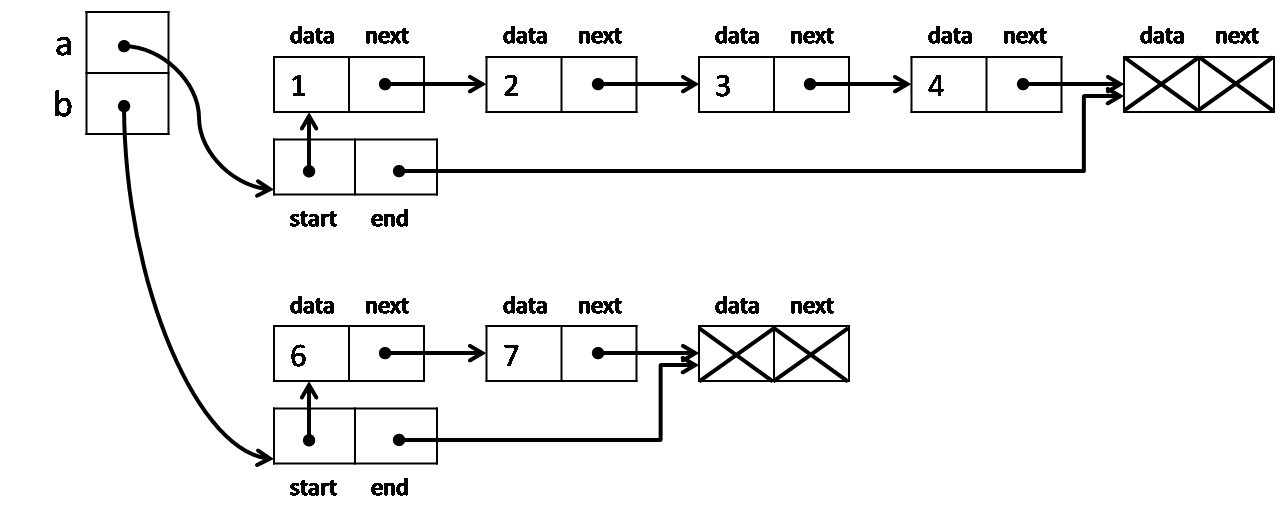
\includegraphics[scale=0.55]{\img/linked1.png}
\end{center}
\vspace*{-2ex}%
\begin{framed}
\ifprintanswers{\color{\answerColor}
  a: 1->6->2->7->3->4->X

  \medskip
  b: X
}\else~\vspace{1.5in}\fi
\end{framed}


\bigskip
\begin{center}
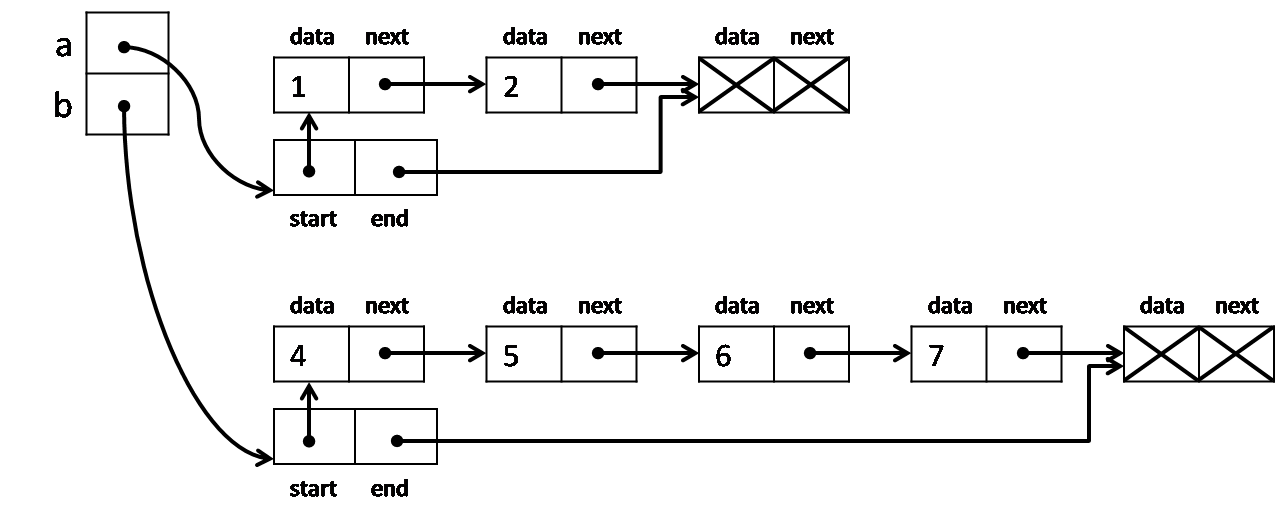
\includegraphics[scale=0.55]{\img/linked2.png}
\end{center}
\vspace*{-2ex}%
\begin{framed}
\ifprintanswers{\color{\answerColor}
  a: 1->4->2->5->X

  \medskip
  b: 6->7->X
}\else~\vspace{1.5in}\fi
\end{framed}

\enlargethispage{5ex}
\medskip
What is the final length of linked list \lstinline'a' when

\noindent
\begin{minipage}[t]{0.45\linewidth}
  \centering $\bullet \quad m \ge n$
  \begin{framed}
    \medskip
    \answer{14em}{$m+n$}
  \end{framed}
\end{minipage}
\hfill
\begin{minipage}[t]{0.45\linewidth}
\centering $\bullet \quad m < n$
  \begin{framed}
    \medskip
    \answer{14em}{$2m$}
  \end{framed}
\end{minipage}

\RUBRIC
Part (c)
TAGS: linked-list, testing

Gradescope rubric:
+0.15pt: a and b are two distinct lists, both of which are valid
+0.35pt: EITHER box 1 contains a: 1->6->2->7->3->4->X,  b: X
+0.15pt: OR    box 1 has at most one pair of mistakes

+0.15pt: a and b are two distinct lists, both of which are valid
+0.35pt: EITHER box 2 contains a: 1->4->2->5->X, b: 6->7->X
+0.15pt: OR    box 2 has at most one pair of mistakes

+0.25pt: First box: m+n
+0.25pt: Second box: 2m
-0.1pt:  Off by one on either
Commentary: (none)

ENDRUBRIC
  %% Optional % S19 S18
\newpage
\part[1\half]\TAGS{linked-correctness, list, safety}
Complete the function below that removes the maximum integer from a
non-empty linked list of integers.  The specification function
\lstinline'gt_listseg(x,s,e)' checks that \lstinline'x' is strictly
larger than every element in the list segment between \lstinline's'
inclusive and \lstinline'e' exclusive.  You may assume there are no
duplicate elements. (Note that loop invariants are not given so we
can't reason about the safety of the code.)

\begin{framed}
\begin{lstlisting}[aboveskip=0pt,belowskip=0pt]
int remove_max(linkedlist a) {

  //@requires [*\uanswer{16.8em}{a != NULL \&\& a->start != a->end}*];  // List not empty
  //@requires is_segment(a->start, a->end);
  //@ensures  is_segment(a->start, a->end);
  //@ensures gt_listseg(\result, a->start, a->end);

  list* first = a->start;
  list* curr = first->next;
  list* prev = first;
  list* max = first;
  list* max_prev = first;

  while ([*\uanswer{30em}{curr != a->end}*]) {
    if (curr->data > max->data) {

       max_prev = [*\uanswer{26em}{prev}*];

       max = [*\uanswer{29em}{curr}*];
    }
    prev = [*\uanswer{30.2em}{curr}*];

    curr = [*\uanswer{30.2em}{curr->next}*];
  }
  if (max == max_prev)

    [*\uanswer{34.5em}{ a->start = a->start->next}*];

  else [*\uanswer{32.7em}{max\_prev->next = max->next}*];
  return max->data;
}
\end{lstlisting}
\end{framed}

\enlargethispage{5ex}
Explain in one sentence why the second postcondition specified in the
function above is not strong enough to reason that this function
removes and returns the maximum integer from the non-empty linked
list.
\begin{framed}
\bigskip\medskip
\answer{34em}{Because \result{} may not be in the original list.\hfill}
\end{framed}

\RUBRIC
Part (d)
TAGS: linked-correctness, list, safety

Gradescope rubric:
+0.1pt  //@requires a != NULL && a->start != a->end;
+0.1pt  while (curr != a->end)
+0.1pt  max_prev = prev;
+0.1pt  max = curr;
+0.1pt  prev = curr;
+0.1pt  curr = curr->next;
+0.2pt  if () a->start = a->start->next;
+0.2pt  else max_prev->next = max->next;
+0.5pt  (2nd box) Because \result may not be in the original list

Commentary:

There are lots of right answers for the a->start = a->start->next line!
Draw it out and check whether the student's answer works!

int remove_max(linkedlist a) {
    //@requires a != NULL;
    //@requires is_segment(a->start, a->end);
    //@ensures  is_segment(a->start, a->end);
    //@ensures gt_listseg(\result, a->start, a->end);

    list* first = a->start;
    list* curr = first->next;
    list* prev = first;
    list* max = first;
    list* max_prev = first;

    while (curr != a->end) {
        if (curr->data > max->data) {
             max_prev = prev;
             max = curr;
        }
        prev = curr;
        curr = curr->next;
    }
    if (max == max_prev)
       a->start = a->start->next;
    else
       max_prev->next = max->next;
    return max->data;
}
ENDRUBRIC
  %% Optional % F19 F18 F17
\end{parts}
